% ============================================================
% Proyecto Final - Estructuras de Datos y Algoritmos (MCD8006)
% Compilar: pdflatex -interaction=nonstopmode Proyecto_Final_Grupo2.tex (x2)
% ============================================================
\documentclass[11pt,letterpaper]{article}

\usepackage[utf8]{inputenc}
\usepackage[spanish]{babel}
\addto\captionsspanish{\renewcommand{\tablename}{Tabla}}
\usepackage{graphicx}
\usepackage{fancyhdr}
\usepackage{geometry}
\usepackage[hidelinks]{hyperref}
\usepackage{booktabs}
\usepackage{listings}
\usepackage{xcolor}
\usepackage{float}
\usepackage{setspace}
\usepackage{enumitem}
\usepackage{caption}
\usepackage{amsmath}
\usepackage{amssymb}
\usepackage{multirow}

\geometry{left=2.0cm, right=2.0cm, top=2.2cm, bottom=2.2cm}
\setlength{\parskip}{3pt}
\setlength{\parindent}{0pt}
\setstretch{1.0}
\setlength{\headheight}{14.5pt}

\pagestyle{fancy}
\fancyhf{}
\fancyhead[L]{Pipeline de Data Streams / Proyecto Final}
\fancyhead[R]{\thepage}
\renewcommand{\headrulewidth}{0.5pt}

\definecolor{codebg}{rgb}{0.95,0.95,0.95}
\definecolor{codeframe}{rgb}{0.8,0.8,0.8}
\lstdefinestyle{mystyle}{
    backgroundcolor=\color{codebg}, frame=single, rulecolor=\color{codeframe},
    basicstyle=\ttfamily\scriptsize, breaklines=true, keepspaces=true,
    showstringspaces=false, tabsize=2, inputencoding=utf8, extendedchars=true,
    literate={á}{{\'a}}1 {é}{{\'e}}1 {í}{{\'i}}1 {ó}{{\'o}}1 {ú}{{\'u}}1 {ñ}{{\~n}}1 {Á}{{\'A}}1 {É}{{\'E}}1 {Í}{{\'I}}1 {Ó}{{\'O}}1 {Ú}{{\'U}}1 {ü}{{\"u}}1 {º}{{\textordmasculine}}1 {¿}{{?`}}1 {¡}{{!`}}1
}
\lstset{style=mystyle}
\newcommand{\code}[1]{\texttt{\detokenize{#1}}}
\graphicspath{{figures/}}
\hypersetup{pdftitle={Proyecto Final de Estructuras de Datos y Algoritmos},pdfauthor={Grupo 2 UTEC}}

\begin{document}

% ============================================================
% CARÁTULA
% ============================================================
\begin{titlepage}
\centering
\vspace*{0.3cm}

\includegraphics[width=4.5cm]{utec-logo.png}\\[0.5cm]
{\Large\bfseries UNIVERSIDAD DE INGENIER\'IA Y TECNOLOG\'IA}\\[0.1cm]
{\large\bfseries ESCUELA DE POSGRADO}\\[1cm]
\rule{\textwidth}{1pt}\\[0.4cm]
{\normalsize\bfseries Estructuras de Datos Avanzadas Orquestadas para un Pipeline Eficiente de Procesamiento de Data Streams}\\[0.1cm]
{\normalsize\bfseries Pipeline de 10 etapas para comercio electr\'onico (escenario B) con 10 millones de eventos de REES46}\\[0.4cm]
\rule{\textwidth}{1pt}\\[1.2cm]
\vfill
{\normalsize\bfseries AUTOR(ES)}\\[0.3cm]
\begin{tabular}{l}
Sebastian Rodrigo Garcia Villacorta\\
Dante Guillermo Barreto Daza\\
Clinton Michael Chulluncuy Reynoso\\
Ronald Ramiro Hilario Orihuela
\end{tabular}\\[0.6cm]
{\normalsize\bfseries DOCENTE}\\[0.2cm]
{\normalsize Heider S\'anchez}\\[0.6cm]
{\normalsize\bfseries CURSO}\\[0.2cm]
{\normalsize Estructuras de Datos y Algoritmos (MCD8006)}\\[0.6cm]
{\normalsize\bfseries REPOSITORIO}\\[0.2cm]
{\normalsize \url{https://github.com/UTEC-AII/Proyecto-Final-E-AD}}\\[1cm]
\vfill
{\normalsize Lima --- Per\'u, 2026}
\end{titlepage}

% ============================================================
\section*{Resumen}
\addcontentsline{toc}{section}{Resumen}

Se construy\'o un pipeline de diez etapas que procesa de punta a punta 10,223,169 eventos de comercio electr\'onico (los primeros diez millones de octubre de 2019 del dataset REES46 y el componente de stream sint\'etico que exige el enunciado) a 33,107 eventos por segundo en Python, con todas las estructuras implementadas desde cero: cola FIFO enlazada, merge sort con b\'usqueda binaria, heap binario, tabla hash, cach\'e LRU, matriz dispersa, B+Tree en disco, KD-Tree, Bloom Filter, Count-Min Sketch, MinHash con LSH, IVF, HNSW, PageRank, Louvain, Label Propagation y Trie. La salida de cada etapa es la entrada real de la siguiente y se verifica con la traza de un evento por las diez etapas y con una prueba de integraci\'on autom\'atica. Repositorio: \url{https://github.com/UTEC-AII/Proyecto-Final-E-AD}.

Los experimentos de 1K a 10M confirman en escala log-log las complejidades te\'oricas. El B+Tree responde una b\'usqueda sobre 10M claves en 44 $\mu$s con altura 3; el KD-Tree resuelve KNN 537 veces m\'as r\'apido que la fuerza bruta en tres dimensiones; LSH responde consultas de casi duplicados 295 veces m\'as r\'apido que la comparaci\'on exhaustiva; IVF, 226 veces frente al KNN exacto en 32 dimensiones con \emph{recall}@10 de 0,95; y el Bloom Filter ocupa 12 MB donde la tabla hash exacta necesita 268 MB, con una tasa de falsos positivos de 1,01 \% frente al 1 \% te\'orico.


% ============================================================
\section{Contexto y objetivo}

Una tienda en l\'inea recibe un flujo continuo de vistas, carritos y compras. Sobre ese flujo hay que priorizar \'ordenes urgentes, consultar productos con baja latencia, detectar fraude en segundos, recomendar productos relacionados y descubrir qu\'e se compra junto. Cada problema tiene una estructura de datos adecuada; el objetivo del proyecto es encadenarlas de modo que la salida de cada etapa sea la entrada real de la siguiente, y medir cu\'anto ganan las estructuras aproximadas frente a sus alternativas exactas.

El enunciado no eval\'ua implementaciones aisladas sino la integraci\'on verificable. Por eso el dise\~no se apoya en dos decisiones transversales: (i) cada etapa deja una nota en la traza del evento, de modo que se pueda demostrar que el dato atraves\'o las diez etapas, y (ii) las estructuras costosas de construir se refrescan per\'iodicamente, como en un sistema lambda con capa r\'apida y capa por lotes.

% ============================================================
\section{Datos y componente de stream}

\subsection{Dataset real}

Se usa \emph{eCommerce behavior data from multi category store} (REES46, Kaggle), el dataset recomendado por el enunciado para el escenario B: unos 285 millones de eventos de comportamiento de una tienda multicategor\'ia, con las columnas \code{event_time}, \code{event_type}, \code{product_id}, \code{category_id}, \code{category_code}, \code{brand}, \code{price}, \code{user_id} y \code{user_session}. DuckDB lee el archivo \code{2019-Oct.csv} (5,7 GB) en streaming y toma los primeros diez millones de eventos en orden temporal, del 1 al 8 de octubre de 2019:

\begin{lstlisting}[language=SQL]
SELECT event_time::TIMESTAMPTZ, event_type, product_id, category_id,
       category_code, brand, price, user_id,
       COALESCE(user_session, 'sin-sesion-' || user_id) AS user_session
FROM read_csv_auto(['data/raw/2019-Oct.csv'], header=true)
WHERE price > 0
ORDER BY event_time
LIMIT 10000000
\end{lstlisting}

El cat\'alogo se deriva de los mismos eventos (marca, categor\'ia, precio mediano y popularidad), y el grafo de co-compra sale de las sesiones que compraron m\'as de un producto. El embudo queda muy desbalanceado: 95,6 \% de vistas, 2,2 \% de carritos y 2,2 \% de compras, con 120,565 productos y 1,072,341 usuarios.

\subsection{Componente de stream sint\'etico}

Ning\'un dataset p\'ublico trae dispositivos, tarjetas, prioridades, fraude ni duplicados, as\'i que, como pide el enunciado, se generan con semilla fija sobre la base real. La Tabla~\ref{tab:datos} separa lo real de lo sint\'etico.

\begin{table}[H]
\centering
\small
\begin{tabular}{@{}p{6.4cm}p{7.6cm}@{}}
\toprule
\textbf{Real (REES46)} & \textbf{Sint\'etico (generado)} \\
\midrule
Productos, precios, marcas y categor\'ias & Dispositivos, IP y tarjetas \\
Usuarios y sus interacciones & Usuario premium y tipo de env\'io \\
Co-compras y grafo del dominio & Consultas de b\'usqueda \\
Marcas de tiempo & R\'afagas de fraude y duplicados \\
\bottomrule
\end{tabular}
\caption{Origen de cada campo del stream. Las etiquetas de verdad se usan solo para medir, nunca para decidir.}
\label{tab:datos}
\end{table}

El enriquecimiento agrega: uno o dos dispositivos por usuario (30 \% tiene dos), una IP y una tarjeta por usuario, 6 \% de usuarios premium, tipo de env\'io en las compras (express 15 \%, est\'andar 70 \%, programado 15 \%), consultas de b\'usqueda en 30 \% de las vistas, 1,5 \% de eventos reenviados con el mismo \code{event_id} unos segundos despu\'es, y r\'afagas de fraude de 25 a 120 intentos en menos de cinco minutos desde una misma tarjeta, dispositivo e IP. La mitad de las tarjetas fraudulentas se asume ya reportada: esa es la lista negra que carga el Bloom Filter. El total procesado se descompone as\'i: 10,000,000 eventos reales, 72,088 de r\'afagas y 151,081 duplicados.

% ============================================================
\section{Arquitectura del pipeline}

El stream se procesa en lotes de 5,000 eventos. Las etapas incrementales (S0 a S4, S6, S8 y S9) act\'uan sobre cada evento; las estructuras est\'aticas o costosas de construir (KD-Tree, firmas MinHash, SVD con IVF, PageRank y Louvain) se refrescan cada dos millones de eventos y al final. La Figura~\ref{fig:pipeline} muestra el flujo y la Tabla~\ref{tab:etapas} la estructura elegida en cada etapa.

\begin{figure}[H]
\centering
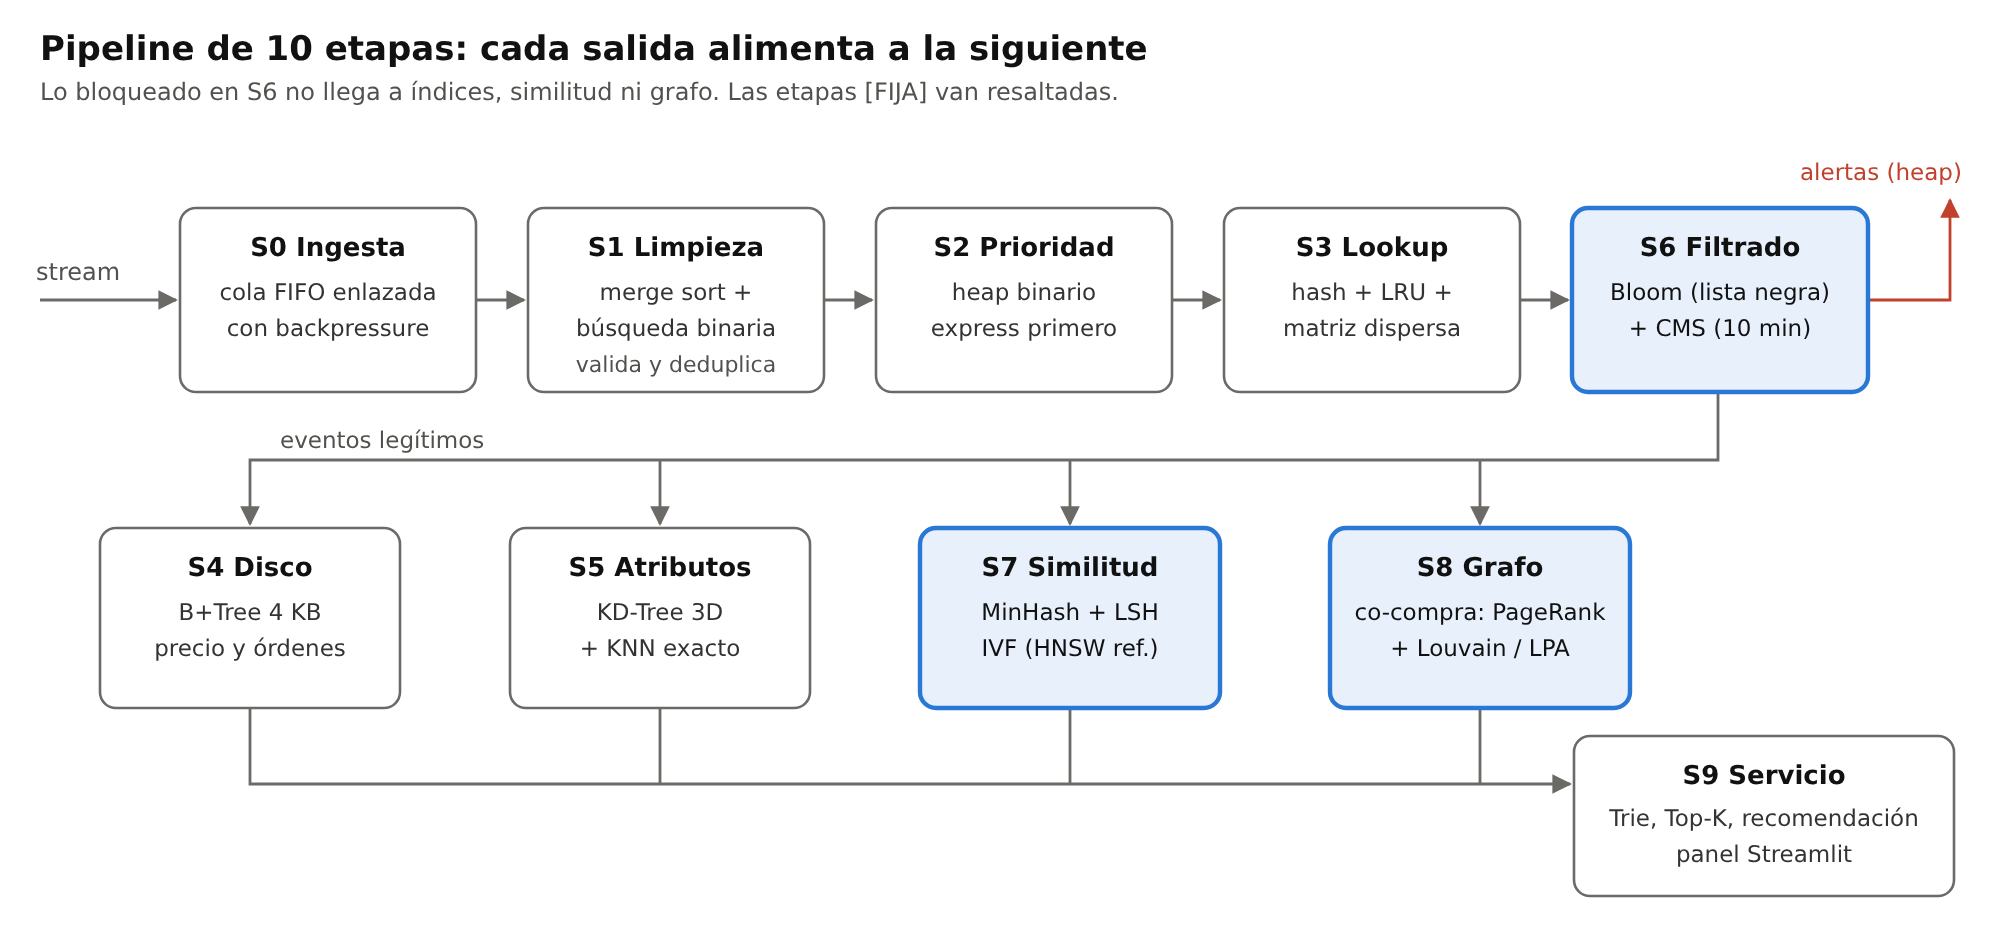
\includegraphics[width=0.95\textwidth]{../docs/pipeline.png}
\caption{Flujo por lote. S6 se ejecuta despu\'es de S3: solo lo que pasa el filtro llega a S4, S5, S7 y S8, y todas las salidas convergen en S9.}
\label{fig:pipeline}
\end{figure}

\begin{table}[H]
\centering
\scriptsize
\resizebox{\textwidth}{!}{%
\begin{tabular}{@{}clp{4.6cm}p{4.2cm}p{3.4cm}@{}}
\toprule
\textbf{Etapa} & \textbf{Estructura} & \textbf{Funci\'on en el pipeline} & \textbf{Complejidad} & \textbf{Alternativa descartada} \\
\midrule
0 & Cola FIFO enlazada acotada & Buffer entre el lector y el consumidor por lotes & enqueue/dequeue $O(1)$ & Lista de Python: \code{pop(0)} es $O(n)$ \\
1 & Merge sort + b\'usqueda binaria en corridas ordenadas & Valida, normaliza, ordena por tiempo y deduplica & $O(b\log b)$ por lote y por corrida solapada & Arreglo \'unico: mezcla $O(W)$; conjunto hash: 1,6$\times$ m\'as lento \\
2 & Heap binario (min-heap) & Compras express, premium, est\'andar, programadas, carritos y vistas & push/pop $O(\log n)$; heapify $O(n)$ & Lista ordenada: inserci\'on $O(n)$ \\
3 & Tabla hash, LRU y matriz dispersa DOK$\to$CSR & Resuelve \code{product_id} y \code{user_id}; cachea fichas; matriz usuario$\times$producto & $O(1)$ amortizado; CSR con $nnz$ & Matriz densa: $200K\times200K$ no cabe \\
4 & B+Tree con p\'aginas de 4 KB & \'Indice de precio (carga masiva) e \'indice temporal de \'ordenes & b\'usqueda $O(\log_B n)$; rango $O(\log_B n + k/B)$ & \'Arbol binario: una p\'agina por nodo \\
5 & KD-Tree + KNN exacto & Vecinos por precio, popularidad y conversi\'on & construcci\'on $O(n\log n)$; KNN $O(\log n)$ en $d$ bajo & Fuerza bruta $O(n)$ por consulta \\
6 & Bloom Filter + Count-Min Sketch & Lista negra verificada y conteo de intentos en 10 minutos & $O(k)$ y $O(d)$ por operaci\'on & Conjunto exacto: memoria sin l\'imite \\
7 & MinHash+LSH, IVF y HNSW & Productos con compradores parecidos y vecinos en embeddings & LSH $O(b\log(nb)+c)$; IVF $O(n_{list}d + n_{probe}\,n/n_{list}\,d)$ & Fuerza bruta $O(n\,d)$ por consulta \\
8 & PageRank, Louvain y Label Propagation & Influencia y comunidades en el grafo de co-compra & PageRank $O(iter \cdot m)$; Louvain $\approx O(m\log n)$ & Ranking por grado: no premia la centralidad \\
9 & Trie, Top-K y panel Streamlit & Autocompletado, m\'as vendidos, recomendaci\'on combinada & Trie $O(L)$; Top-K $O(n\log K)$ & Ordenar todo: $O(n\log n)$ \\
\bottomrule
\end{tabular}}
\caption{Estructuras de las diez etapas, su funci\'on y su complejidad.}
\label{tab:etapas}
\end{table}

\subsection*{Sobre el orden de ejecuci\'on}

El enunciado numera el filtrado probabil\'istico como etapa 6, despu\'es del KD-Tree. El pipeline lo ejecuta inmediatamente despu\'es de S3 por una raz\'on de ingenier\'ia: un evento bloqueado no debe actualizar \'indices, similitud ni grafo, y filtrarlo antes evita ese costo. La decisi\'on tiene un costo expl\'icito que se declara: una sobreestimaci\'on del Count-Min descarta un evento leg\'itimo antes de que actualice la matriz de interacciones y el grafo, de modo que las etapas posteriores ven un stream levemente sesgado. Los falsos positivos del Bloom, en cambio, se verifican contra el conjunto exacto antes de bloquear, as\'i que no descartan nada.

% ============================================================
\section{Etapas 0 a 5: estructuras base}

\subsection{S0: Ingesta con cola FIFO acotada}
Cola enlazada con capacidad de un lote. \code{enqueue} y \code{dequeue} cuestan $O(1)$ y no hay desplazamientos de memoria; cuando la cola est\'a llena, \code{enqueue} devuelve falso, el productor se detiene y el evento se contabiliza como rechazo. La alternativa descartada es la lista de Python con \code{pop(0)}, cuyo costo es $O(n)$ por extracci\'on y $O(n^2)$ en un bucle de ingesta. La prueba \code{test\_linked\_queue\_fifo\_and\_capacity} verifica el orden FIFO y el rechazo al llenarse.

\subsection{S1: Preprocesamiento y deduplicaci\'on}
Se valida el evento (tipo v\'alido, producto, usuario, precio positivo y marca de tiempo), se normaliza texto y precio, y se deduplica en dos niveles. Dentro del lote, merge sort por \code{event_id} deja los repetidos adyacentes. Contra la ventana de los \'ultimos 500,000 identificadores, la ventana se guarda como un anillo de corridas ordenadas, una por lote, y cada lote se busca con b\'usqueda binaria vectorizada solo en las corridas cuyo rango $[\min,\max]$ se solapa con el suyo; al llenarse, se descarta la corrida m\'as antigua completa. El costo es $O(b\log b)$ por lote y por corrida solapada, sin la mezcla $O(W)$ de un arreglo \'unico ordenado, y la memoria queda acotada a la ventana. Frente al conjunto hash propio, que es $O(1)$ por evento pero se ejecuta en Python puro, la b\'usqueda binaria vectorizada elimina exactamente los mismos duplicados y es 1,6 veces m\'as r\'apida sobre los 10M de eventos (50 s frente a 79 s en 4 vCPU).

\subsection{S2: Prioridad con heap binario}
Min-heap sobre arreglo con desempate por secuencia de llegada, de modo que dentro de una misma prioridad el orden es FIFO. Las compras se clasifican en express, premium, est\'andar y programadas; luego carritos y vistas. \code{push} y \code{pop} cuestan $O(\log n)$ y \code{heapify} $O(n)$. La alternativa descartada es mantener una lista ordenada, cuya inserci\'on es $O(n)$.

\subsection{S3: Almacenamiento, cach\'e y matriz dispersa}
Tabla hash con sondeo lineal, factor de carga m\'aximo 0,7 y l\'apidas para el borrado, que resuelve \code{product\_id} y \code{user\_id} a \'\i ndices densos en $O(1)$ amortizado. Sobre ella se apoyan la cach\'e LRU (tabla hash m\'as lista doblemente enlazada, $O(1)$ por acceso) y la matriz usuario$\times$producto, que se acumula en formato DOK y se compacta a CSR para el \'algebra matricial. La alternativa descartada es la matriz densa: $200K\times200K$ en doble precisi\'on no cabe en memoria.

\subsection{S4: \'Indice principal en disco}
B+Tree de p\'aginas de 4 KB con hojas enlazadas y b\'uffer de p\'aginas con escritura diferida. Los datos viven solo en las hojas y las claves internas son separadores, lo que maximiza el abanico y permite recorrer rangos sin volver a subir por el \'arbol. Para 10 M de claves con 255 entradas por hoja y una ocupaci\'on del 90 \% resultan 43,862 hojas, 171 p\'aginas internas y una ra\'iz: altura 3, es decir tres p\'aginas por b\'usqueda y $O(\log_B n + k/B)$ por rango.

La comparaci\'on con un \'arbol binario es la que justifica la elecci\'on: un nodo AVL ocupa unos 40 bytes y el disco transfiere p\'aginas de 4 KB, as\'i que leer un nodo desperdicia m\'as del 99 \% de la p\'agina. Para $10^9$ claves un AVL necesitar\'ia unos 43 accesos a disco (del orden de 430 ms) mientras que el B+Tree necesita cuatro (unos 40 ms). El \'indice temporal de \'ordenes se llena con marcas de tiempo crecientes, el patr\'on que la teor\'ia se\~nala como peligroso para un BST: el B+Tree lo absorbe porque se balancea solo, aunque las hojas quedan alrededor del 50 \% de ocupaci\'on.

\subsection{S5: \'Indice multidimensional y KNN exacto}
KD-Tree construido por corte en la mediana del eje m\'as extendido, con hojas de 16 puntos, sobre tres atributos normalizados: logaritmo del precio, logaritmo de las vistas y tasa de conversi\'on. La construcci\'on es $O(n\log n)$ y la consulta $O(\log n)$ en dimensi\'on baja. En 32 dimensiones el \'arbol deja de podar y resulta 421 veces m\'as lento que la fuerza bruta, que es exactamente la maldici\'on de la dimensionalidad: por eso los embeddings se buscan con IVF y no con KD-Tree.

% ============================================================
\section{Bloque de investigaci\'on avanzada (etapas 6 a 8)}

\subsection{Filtrado probabil\'istico: Bloom Filter y Count-Min Sketch}
\textbf{Bloom Filter} (Bloom, 1970). Arreglo de $m$ bits y $k$ funciones hash; insertar enciende $k$ bits y consultar responde \emph{posiblemente presente} si los $k$ est\'an encendidos. No hay falsos negativos y la tasa de falsos positivos es
\begin{equation}
p \approx \left(1-e^{-kn/m}\right)^{k}, \qquad m = -\frac{n\ln p}{(\ln 2)^2}, \qquad k = \frac{m}{n}\ln 2,
\end{equation}
de modo que para $p=1$ \% bastan 9,59 bits por elemento y $k=7$, sin importar el tama\~no de la clave. Las $k$ posiciones se generan con doble hashing $g_i = h_1 + i\,h_2 \bmod m$ (Kirsch y Mitzenmacher, 2006) sobre \code{splitmix64}, y los bits van empaquetados en \code{uint8}. Uso: lista negra de tarjetas y dispositivos. Como un positivo puede ser falso y bloquear una compra es una decisi\'on cr\'itica, todo positivo se verifica contra el conjunto exacto. L\'imites: no admite borrado (s\'i con contadores, \emph{Counting Bloom}) y la tasa crece si se supera la capacidad.

\textbf{Count-Min Sketch} (Cormode y Muthukrishnan, 2005). Matriz de $d\times w$ contadores con un hash por fila; la estimaci\'on es el m\'inimo de las $d$ celdas. Nunca subestima y, con $w=\lceil e/\varepsilon\rceil$ y $d=\lceil\ln(1/\delta)\rceil$, cumple $\hat{f} \le f + \varepsilon N$ con probabilidad $1-\delta$. La memoria $O(wd)$ no depende del n\'umero de claves. Uso: intentos de compra o carrito por tarjeta y por dispositivo en una ventana de 10 minutos, implementada como anillo de 10 sub-sketches de un minuto que se limpia al avanzar. El umbral es de m\'as de 12 intentos por tarjeta o 20 por dispositivo dentro de la ventana; como solo puede sobreestimar, una alerta puede adelantarse pero nunca ocultarse.

\subsection{Similitud de conjuntos: MinHash y LSH}
Para una permutaci\'on aleatoria $h$, $\mathbb{P}[\min h(A)=\min h(B)] = J(A,B)$ (Broder, 1997): la fracci\'on de coincidencias entre dos firmas de $P$ minhashes estima el \'indice de Jaccard con error est\'andar $\sqrt{J(1-J)/P}$. Con LSH por bandas la firma se corta en $b$ bandas de $r$ filas y dos conjuntos son candidatos si coinciden en una banda completa:
\begin{equation}
\mathbb{P}[\text{candidato}] = 1-\left(1-J^{r}\right)^{b}, \qquad \text{umbral} \approx \left(1/b\right)^{1/r}.
\end{equation}
Se eligi\'o MinHash y no SimHash porque el objeto natural es un conjunto: los usuarios que pusieron cada producto en el carrito o lo compraron. Con $P=128$, $b=32$ y $r=4$ el umbral es 0,42. Las 32 bandas se indexan en un arreglo ordenado de pares y una consulta son dos b\'usquedas binarias vectorizadas. Conviene ser expl\'icitos sobre su alcance: LSH es un detector de casi duplicados, no un \'indice de vecinos globales; admite falsos negativos, y por eso el \emph{recall} se reporta de dos formas en la Secci\'on~\ref{sec:similitud}. Para vecinos en el espacio completo se usa IVF.

\subsection{B\'usqueda aproximada de vecinos: IVF y HNSW}
Los productos se representan con embeddings de 32 dimensiones obtenidos por SVD truncada aleatorizada (Halko et al., 2011) de la matriz usuario$\times$producto en CSR, implementada solo con productos matriz-vector. IVF (J\'egou et al., 2011) divide el espacio con k-means++ y Lloyd en $n_{list}=4\sqrt{n}$ celdas (m\'aximo 4096) y una consulta recorre las $n_{probe}$ listas m\'as cercanas, con costo $O(n_{list}d + n_{probe}(n/n_{list})d)$. HNSW (Malkov y Yashunin, 2020) es un grafo navegable en capas con descenso voraz y b\'usqueda \emph{best-first} con $ef$ candidatos. Se eligi\'o IVF para el pipeline porque su construcci\'on y consulta son operaciones de matriz y escala en Python; HNSW se implement\'o para comparar el compromiso entre \emph{recall} y latencia. La l\'inea base es el KNN exacto por fuerza bruta, $O(nd)$.

\subsection{Ranking de influencia: PageRank}
El grafo de co-compra es no dirigido y ponderado: nodos son productos y $w(u,v)$ es el n\'umero de \'ordenes que contienen a ambos. PageRank (Brin y Page, 1998) es el vector estacionario de una caminata aleatoria que sigue aristas con probabilidad proporcional al peso y salta a un nodo aleatorio con probabilidad $1-\alpha$:
\begin{equation}
r \leftarrow \alpha P^{\top} r + \alpha\left(\sum_{j \in \text{colgantes}} r_j\right) v + (1-\alpha)v .
\end{equation}
Se implementa con iteraci\'on de potencias sobre la CSR ($O(m)$ por iteraci\'on) hasta que el cambio en norma $L_1$ baja de $10^{-9}$, y se valida contra NetworkX. La l\'inea base es el grado ponderado; PageRank premia estar conectado con productos que a su vez son centrales, no solo tener muchas co-compras.

\subsection{Comunidades: Louvain frente a Label Propagation}
Louvain (Blondel et al., 2008) maximiza la modularidad
\begin{equation}
Q = \sum_c \left[\frac{L_c}{2m} - \left(\frac{d_c}{2m}\right)^2\right]
\end{equation}
en dos fases repetidas: mover cada nodo a la comunidad vecina con mayor ganancia $\Delta Q \propto k_{i,c} - \Sigma_{tot}k_i/2m$, y colapsar cada comunidad en un nodo; su costo es casi $O(m\log n)$. Label Propagation (Raghavan et al., 2007) adopta la etiqueta de mayor peso entre los vecinos: es casi lineal pero no optimiza una funci\'on objetivo, por lo que es menos estable. La estabilidad se mide con informaci\'on mutua normalizada entre corridas con distinta semilla. Leiden (Traag et al., 2019) corrige comunidades mal conectadas de Louvain y queda como trabajo futuro.

% ============================================================
\section{Dise\~no de la integraci\'on}

La integraci\'on se verifica con un evento concreto. En la corrida de 10M se traz\'o autom\'aticamente una compra leg\'itima ubicada al 70 \% del stream; la Figura~\ref{fig:traza} muestra su salida literal. Es la compra de un Samsung de 131,76 USD, el producto con mayor PageRank del grafo. Tiene env\'io programado, as\'i que el heap la deja en la posici\'on 89 de 4,929, detr\'as de las compras express, premium y est\'andar del lote. LSH no devolvi\'o candidatos porque ning\'un producto supera el umbral de Jaccard de 0,42 con su conjunto de compradores; la recomendaci\'on final combina el grafo de co-compra, el KD-Tree (smartphones de la misma marca y rango de precio) y el IVF, y deja registrada la fuente de cada producto.

\begin{figure}[H]
\centering
\begin{lstlisting}[language=Python, basicstyle=\ttfamily\scriptsize]
Event(id=6967856, purchase, product=1004856, user=528344847, price=131.76)
[S0] encolado (cola=2366)
[S1] valido, normalizado y no duplicado
[S2] prioridad 3 (compra programada), posicion 89 de 4929 en el lote
[S3] producto #861 y usuario #746725 resueltos en la tabla hash
[S6] pasa el filtro (Bloom: ausente; CMS bajo el umbral)
[S4] orden indexada por tiempo en el B+Tree
[S5] vecinos por atributos (KD-Tree): [786, 840, 14608]
[S7] LSH: []; vecinos IVF: [87862, 87190, 40728]
[S8] primera compra de la orden: nodo listo para nuevas aristas
[S9] Top-5: samsung 4767 (1.687, grafo+KD) ... samsung 4836 (0.952, grafo)
\end{lstlisting}
\caption{Recorrido de un evento por las diez etapas en la corrida de 10M.}
\label{fig:traza}
\end{figure}

Cada flecha de la Figura~\ref{fig:pipeline} corresponde a un dato que la etapa siguiente consume: los \'\i ndices densos de S3 son las filas y columnas de la matriz dispersa y los nodos del grafo; la matriz alimenta las firmas MinHash y la SVD de S7; las aristas de co-compra de S8 y su PageRank ponderan el ranking de S9, que adem\'as usa los vecinos del KD-Tree y cachea el resultado en el LRU. Las alertas de S6 se ordenan en un heap por severidad (lista negra antes que frecuencia) y las etiquetas de verdad se usan solo para medir.

% ============================================================
\section{Experimentaci\'on y an\'alisis}
\label{sec:experimentos}

\subsection{Metodolog\'ia}
Se usan tama\~nos de 1K a 10M con 100 repeticiones para 1K y 10K, 10 para 100K, 3 para 1M y 1 para 10M (con 100 repeticiones la serie de 10M habr\'ia tomado d\'ias en Python puro). Se reporta la media y la desviaci\'on est\'andar, el pico de memoria con \code{tracemalloc} y la pendiente en escala log-log como exponente emp\'irico. Semilla fija 2026; plataforma de 4 vCPU y 16 GB, Python 3.13 y NumPy 2.5.4 (\code{results/bench/platform.json}). Los experimentos de escalabilidad usan entradas generadas para controlar $n$ y conocer la respuesta exacta; la corrida del pipeline usa los datos reales.

\subsection{Estructuras base}
La Figura~\ref{fig:escala} muestra el tiempo total frente a $n$ en escala log-log. Las pendientes medidas siguen la teor\'ia: lineal en la cola y la tabla hash (1,12 y 1,08), $n\log n$ en la ordenaci\'on y el heap (1,21 y 1,22), casi constante en la b\'usqueda del B+Tree (0,32) y en el KNN del KD-Tree en tres dimensiones (0,11), y lineal en todas las l\'ineas base de fuerza bruta (1,02).

\begin{figure}[H]
\centering
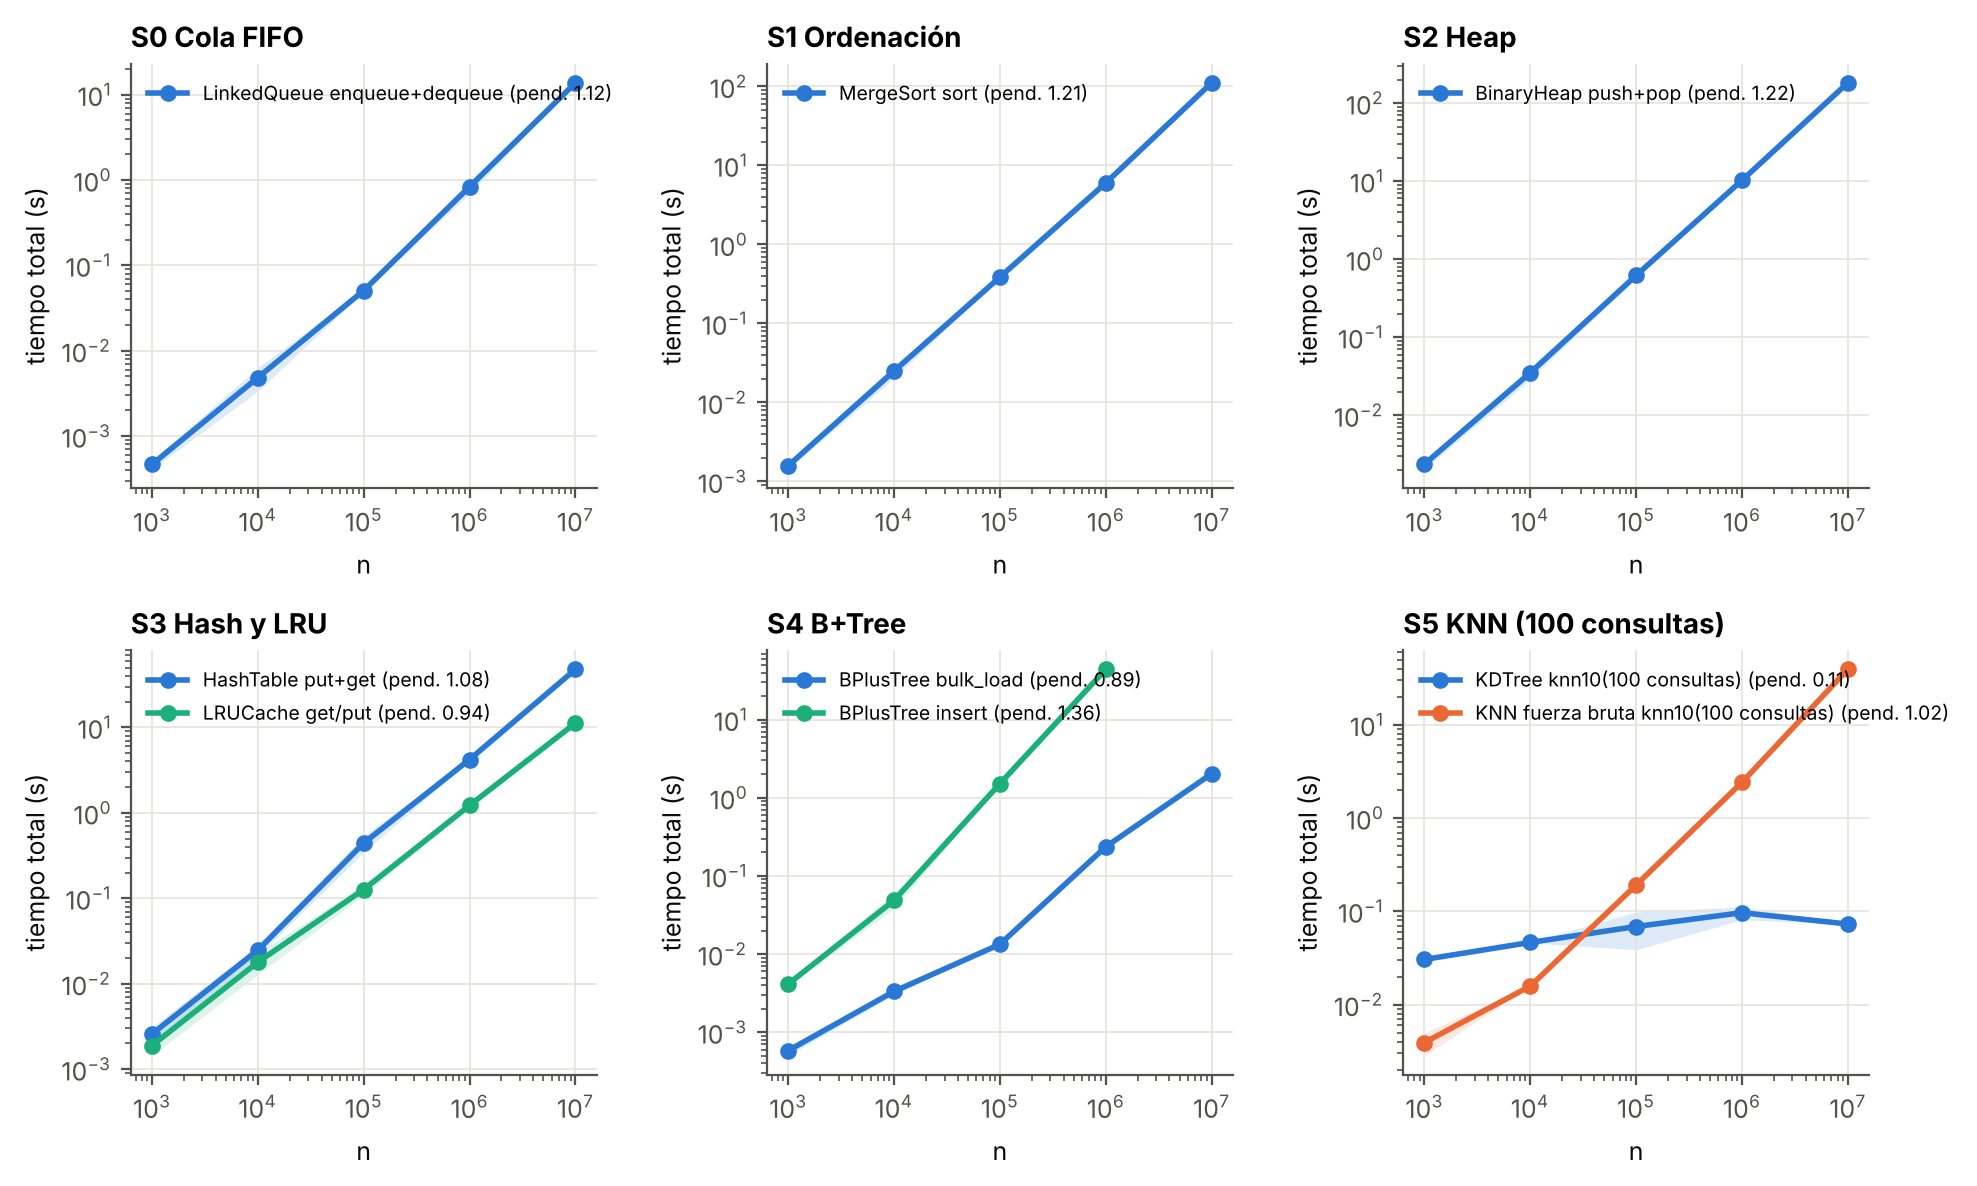
\includegraphics[width=0.82\textwidth]{fig_base_scaling.png}
\caption{Tiempo total frente a $n$ (log-log), de 1K a 10M operaciones. La pendiente ajustada aparece en la leyenda.}
\label{fig:escala}
\end{figure}

\begin{table}[H]
\centering
\scriptsize
\resizebox{\textwidth}{!}{%
\begin{tabular}{@{}lrrrrl@{}}
\toprule
\textbf{Estructura ($n=10$M)} & \textbf{Tiempo total} & \textbf{Por oper.} & \textbf{Pendiente} & \textbf{Memoria (1M)} & \textbf{Observaci\'on} \\
\midrule
Cola FIFO (enqueue+dequeue) & 13,7 s & 0,69 $\mu$s & 1,12 & 45,8 MB & Lineal, como se espera \\
Merge sort & 111 s & 11,1 $\mu$s & 1,21 & 61,5 MB & El factor $\log n$ eleva la pendiente \\
Heap binario (push+pop) & 181 s & 9,1 $\mu$s & 1,22 & 107,2 MB & $O(n\log n)$ en total \\
Tabla hash (put+get) & 47,9 s & 2,4 $\mu$s & 1,08 & 48,0 MB & 2,11 sondeos por operaci\'on con carga $\le 0{,}7$ \\
Cach\'e LRU & 11,2 s & 1,1 $\mu$s & 0,94 & 10,1 MB & 91,5 \% de aciertos con accesos Zipf \\
B+Tree: carga / b\'usqueda & 2,0 s / 44,4 $\mu$s & 0,20 / 44,4 $\mu$s & 0,89 / 0,32 & 17,1 MB & Archivo a 1M; a 10M, altura 3 y 43,862 p\'aginas \\
KD-Tree: KNN ($k=10$) & 0,73 ms & n/d & 0,11 & 71,5 MB & 537 veces m\'as r\'apido que la fuerza bruta (393 ms) \\
Fuerza bruta: KNN ($k=10$) & 393 ms & n/d & 1,02 & 38,2 MB & L\'inea base exacta \\
\bottomrule
\end{tabular}}
\caption{Estructuras base con $n=10$M. La memoria pico se midi\'o con \code{tracemalloc} a 1M de elementos (su costo crece linealmente con $n$); en el B+Tree se reporta el tama\~no del archivo.}
\label{tab:base}
\end{table}

\subsection{Filtrado probabil\'istico}
El Bloom Filter se compar\'o con la tabla hash exacta propia y con el \code{set} de Python. Con 10M elementos el Bloom ($p=1$ \%) ocupa 12 MB frente a 268 MB de la tabla exacta (22 veces menos) y es 4,8 veces m\'as r\'apido en inserci\'on y consulta. La tasa medida de falsos positivos coincide con la te\'orica en los tres valores de $p$ (0,0935 \% frente a 0,1000 \% con $p=0{,}1$ \%; 1,01 \% frente a 1,00 \% con $p=1$ \%), y no hubo un solo falso negativo.


Con 10M actualizaciones sobre 1M claves, el Count-Min con $\varepsilon=0{,}001$ usa 53 KB frente a 16,8 MB y actualiza 4,6 veces m\'as r\'apido. El error medio (642) y el m\'aximo (4,146) quedan bajo la cota $\varepsilon N = 9,997$ en el 100 \% de las claves, sin subestimar nunca; para las claves frecuentes, que son las que disparan alertas, el error relativo es 4 \%.

\subsection{Similitud y b\'usqueda de vecinos}
\label{sec:similitud}
La consulta LSH se mantiene entre 0,6 y 0,8 ms de 1K a 1M conjuntos (pendiente 0,05), mientras la fuerza bruta crece linealmente hasta 225 ms: LSH es 295 veces m\'as r\'apido en 1M. El costo est\'a en la construcci\'on (98 s para 1M) y en la memoria de las firmas (1,5 GB), por eso se omiti\'o 10M.

Sobre el \emph{recall} conviene reportar las dos lecturas, porque LSH no es un \'indice de vecinos globales. Sobre los vecinos relevantes (Jaccard $\ge 0{,}5$) el recall@10 es 1,0; sobre el top-10 completo es 0,029, con 1,33 candidatos por consulta. Es el comportamiento esperado de un detector de casi duplicados con umbral 0,42: acierta lo que est\'a por encima del umbral y descarta lo que est\'a lejos. Para vecinos en el espacio completo se usa IVF, que s\'i se eval\'ua contra el KNN exacto: con 10M vectores de 32 dimensiones responde en 0,46 ms frente a 104 ms del KNN exacto (226 veces) con recall@10 de 0,95; con $n_{probe}=16$ sube a 0,98 a la mitad de velocidad. El \'indice ocupa 1,36 GB frente a 1,28 GB de los vectores: un 6 \% m\'as de memoria por 226 veces menos tiempo. En 1M, el barrido de $n_{probe}$ de 1 a 32 recorre la curva de recall de 0,23 a 0,99. HNSW en Python puro lleg\'o a recall 0,97 en 10K pero a 0,80 en 100K con $ef$ de 50 a 100, y su construcci\'on tard\'o 316 s en 100K, por lo que se limit\'o a 100K.

\begin{figure}[H]
\centering
\begin{minipage}{0.49\textwidth}\centering
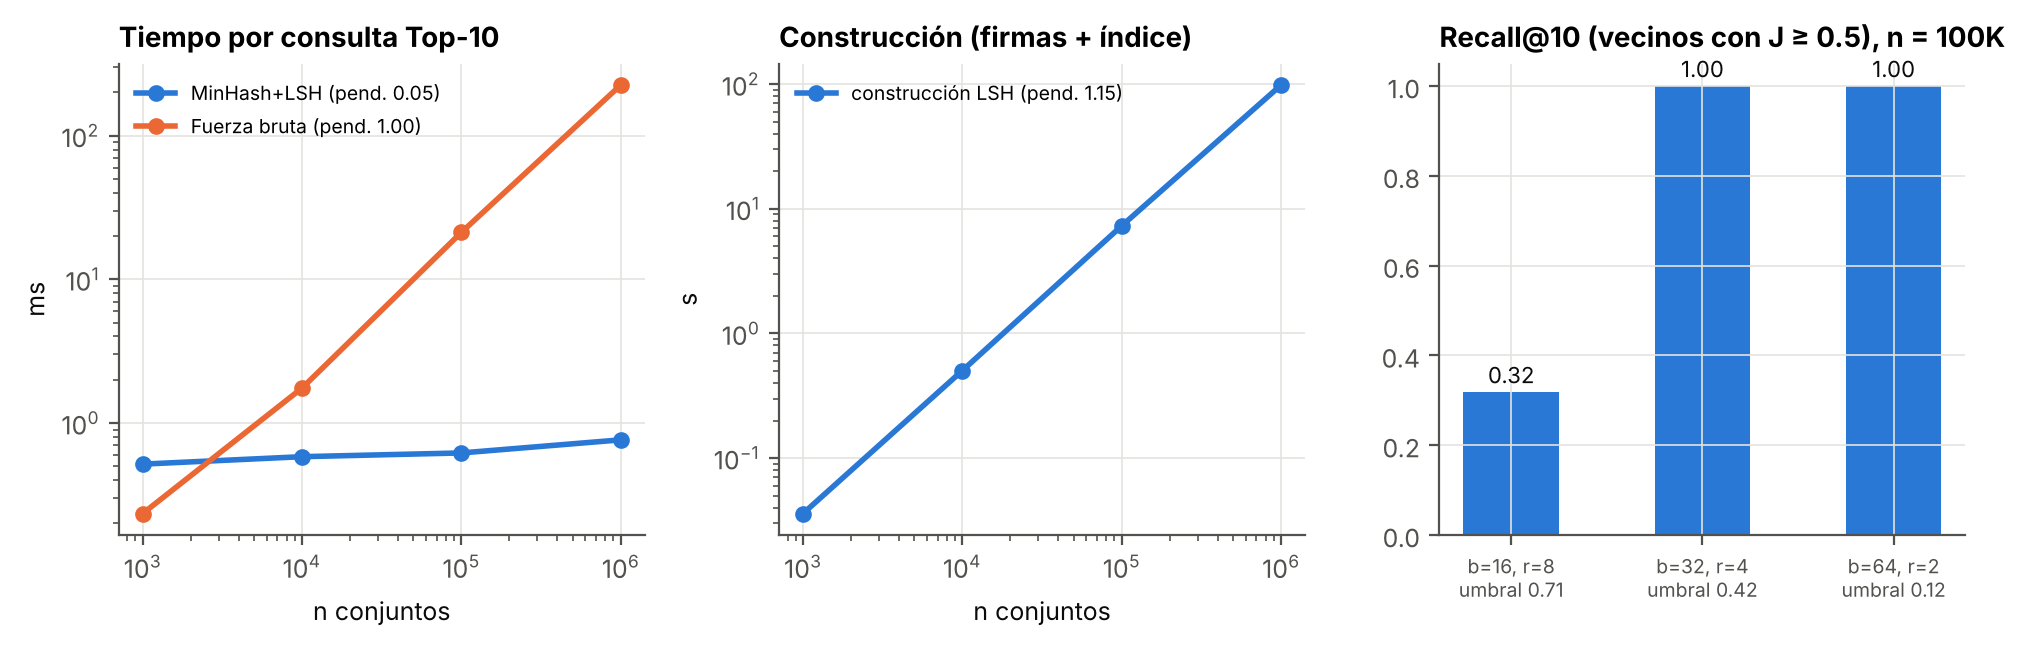
\includegraphics[width=\textwidth]{fig_minhash.png}
\end{minipage}\hfill
\begin{minipage}{0.49\textwidth}\centering
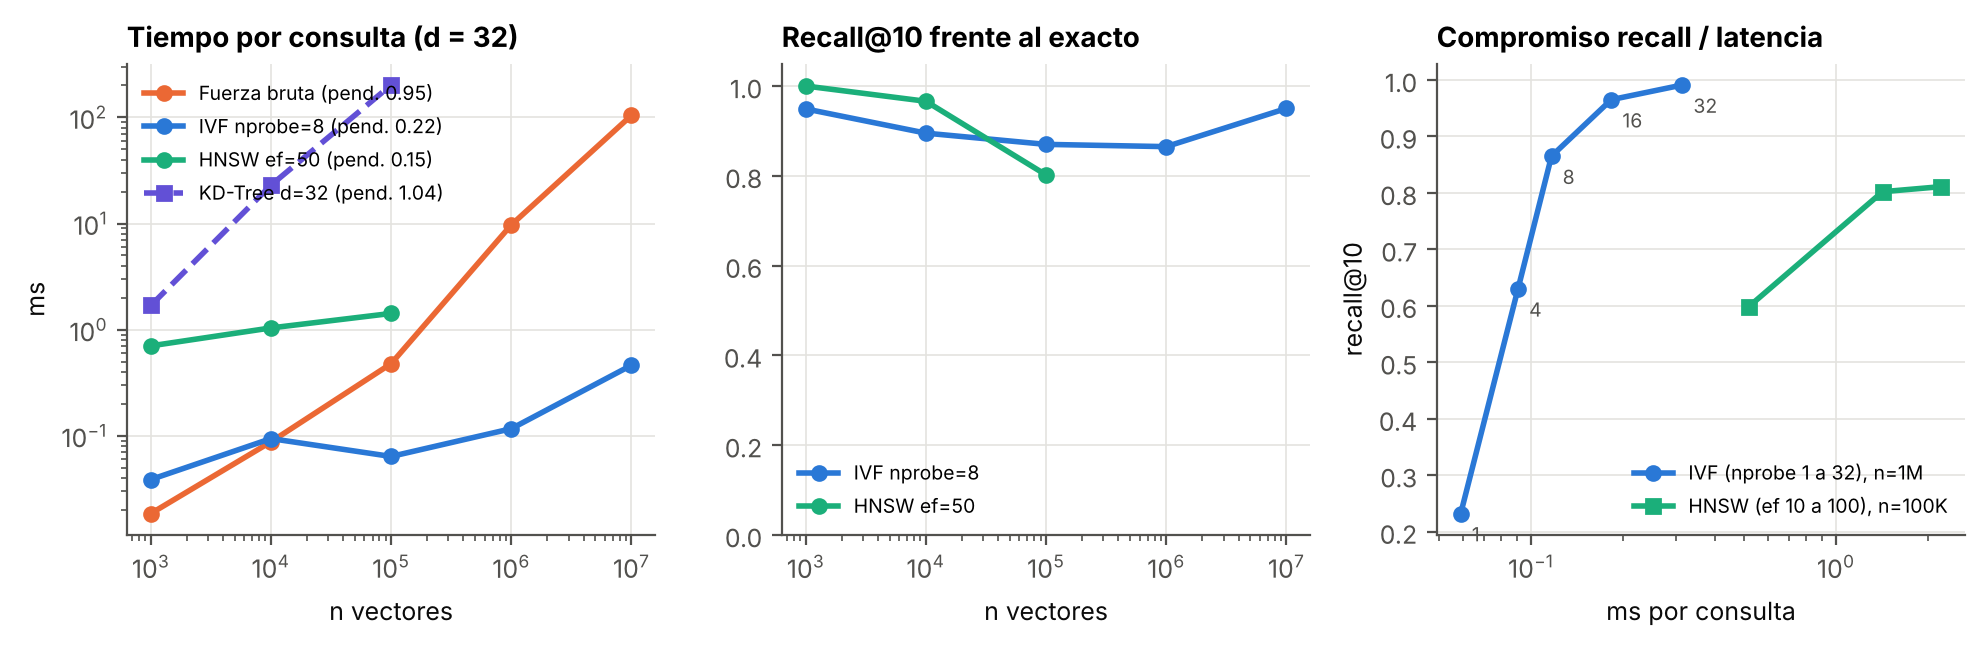
\includegraphics[width=\textwidth]{fig_ann.png}
\end{minipage}
\caption{Izquierda: MinHash+LSH frente a Jaccard exacto. Derecha: IVF y HNSW frente a KNN exacto y al KD-Tree en $d=32$.}
\label{fig:sim}
\end{figure}

Sin aproximaci\'on, el KD-Tree en $d=32$ fue 421 veces m\'as lento que la fuerza bruta en 100K, porque en alta dimensi\'on casi no poda ramas: es la evidencia emp\'irica de la maldici\'on de la dimensionalidad.

\subsection{Grafo de co-compra}
PageRank escala linealmente en aristas (pendiente 1,08) y converge en 47 a 56 iteraciones: 20,7 s para 9,9M aristas. Su correlaci\'on de Spearman con el grado ponderado es 0,99 y el top-100 coincide en 97 \%, as\'i que en co-compra la diferencia est\'a en la cola: PageRank sube productos conectados con productos centrales.

En comunidades, sobre grafos con particiones plantadas, Louvain obtiene mayor modularidad que Label Propagation en todos los tama\~nos (0,781 frente a 0,750 con 1M aristas, igual a la partici\'on plantada), es m\'as estable entre semillas (NMI 0,99 frente a 0,94) y recupera mejor la partici\'on real (NMI 0,96 frente a 0,93), aunque tarda 25 s frente a 19 s. Con 10M aristas solo corri\'o LPA (448 s), que se fragment\'o en 104,606 comunidades con $Q=0,68$; Louvain en Python puro super\'o los 40 minutos y se acot\'o a 1M aristas. En el grafo real de co-compra, que es peque\~no y disperso porque pocas sesiones compran m\'as de un producto (6,921 productos y 14,176 aristas), Louvain logr\'o $Q=0,621$ con 1,005 comunidades frente a $Q=0,383$ de LPA con 1,621.


% ============================================================
\section{Corrida completa y correcciones de la versi\'on final}

\subsection{Corrida con 10M de eventos}\label{sec:corrida}
La Tabla~\ref{tab:corrida} resume la corrida de punta a punta sobre los 10,223,169 eventos. El total fue de 308,8 s (33,107 eventos por segundo) en un Apple M5 de 10 n\'ucleos y 16 GB con Python 3.14, en un solo proceso. Se eliminaron los 151,081 duplicados inyectados sin falsos positivos, se indexaron 179,043 \'ordenes en el B+Tree en disco y la matriz usuario$\times$producto acumul\'o 5,8 millones de celdas no nulas. El filtro de S6 bloque\'o 66,628 eventos con 95,4 \% de precisi\'on y 88,1 \% de exhaustividad; de los 34,434 positivos del Bloom, 7 eran falsos y se descartaron con la verificaci\'on exacta. El refresco de S7 concentra el 49 \% del tiempo (SVD y k-means sobre la matriz completa); refrescar con menor frecuencia o en paralelo es la mejora m\'as directa.

\begin{table}[H]
\centering
\small
\begin{tabular}{@{}lrlr@{}}
\toprule
\textbf{Etapa} & \textbf{Tiempo (s)} & \textbf{Etapa} & \textbf{Tiempo (s)} \\
\midrule
S0 ingesta (lectura Parquet + cola) & 58,2 & S4 B+Tree & 0,8 \\
S1 preprocesamiento & 29,5 & S5 KD-Tree y refresco & 0,7 \\
S2 prioridad & 20,1 & S7 refresco LSH + SVD + IVF & 151,0 \\
S3 almacenamiento e interacciones & 24,7 & S8 grafo y refrescos & 1,1 \\
S6 filtrado & 18,7 & S9 servicio & 1,8 \\
\midrule
\multicolumn{3}{@{}l}{\textbf{Total} (10,223,169 eventos)} & \textbf{308,8} \\
\bottomrule
\end{tabular}
\caption{Tiempo por etapa en la corrida con los 10M eventos reales.}
\label{tab:corrida}
\end{table}

\subsection{Correcciones aplicadas}
\label{sec:correcciones}
La revisi\'on del c\'odigo y del informe identific\'o seis defectos que se corrigieron antes de la entrega:

\begin{enumerate}[leftmargin=1.2em]
\item \textbf{S6: marca permanente.} Cuando una tarjeta cruzaba el umbral quedaba bloqueada para siempre, as\'i que la regla dejaba de ser una ventana de diez minutos. Ahora el umbral se eval\'ua siempre sobre la ventana m\'ovil y la tarjeta vuelve a operar cuando su conteo decae. Se reportan las alertas por motivo.
\item \textbf{S1: estructura de deduplicaci\'on.} El arreglo \'unico ordenado obligaba a mezclar del orden de 500 mil identificadores por lote. Un conjunto hash resolv\'ia el costo pero dejaba la etapa sin la b\'usqueda binaria que pide el enunciado. La versi\'on final guarda la ventana como corridas ordenadas por lote y busca con b\'usqueda binaria vectorizada: sin mezclas $O(W)$, con memoria acotada y 1,6 veces m\'as r\'apida que el conjunto hash.
\item \textbf{S0: capacidad de la cola.} El buffer era cuatro veces el lote, de modo que el backpressure nunca se ejerc\'ia. Ahora su capacidad es de un lote, cuenta los rechazos cuando est\'a llena y una prueba unitaria verifica el rechazo.
\item \textbf{S3: corrupci\'on silenciosa de la matriz.} La celda se codificaba como \code{fila*ncols+col}; al crecer el cat\'alogo, las claves ya guardadas se decodificaban corridas. Ahora la clave es el par (fila, columna).
\item \textbf{S5 y S8: corrupci\'on del grafo.} La arista se codificaba como \code{a*n+b} con una dimensi\'on que cambiaba al refrescar. Ahora la arista es el par $(u,v)$ y la dimensi\'on se recalcula al construir la CSR.
\item \textbf{Memoria del benchmark.} Solo dos de ocho estructuras reportaban pico de memoria. El arn\'es mide ahora \code{tracemalloc} para todas, y el B+Tree reporta el tama\~no de su archivo.
\end{enumerate}

Adem\'as se corrigieron tres problemas de documentaci\'on: la Tabla de estructuras base se hab\'ia partido en dos p\'aginas y este informe la rehace en una sola; la secci\'on de las etapas 0 a 5 pas\'o de tres l\'ineas a una subsecci\'on por etapa con funci\'on, complejidad y alternativa; y el \emph{recall} de LSH se reporta ahora con sus dos lecturas (global y sobre vecinos relevantes) en lugar de solo la favorable.

\subsection{Validaci\'on de las correcciones}
Las correcciones se validaron con una corrida completa de la versi\'on final sobre un mill\'on de eventos sint\'eticos (1,022,378 tras inyectar r\'afagas y duplicados), en 27,37 s y 37,358 eventos por segundo. Los 15,109 duplicados se eliminaron todos. El filtro bloque\'o 5,974 eventos con precisi\'on de 100 \% y \emph{recall} de 82,12 \%: el \emph{recall} baja respecto de la versi\'on anterior porque ya no se sostiene con una marca permanente, que es precisamente el sesgo que se corrigi\'o. Las alertas se repartieron en 3,433 por lista negra y 2,541 por frecuencia de tarjeta. El B+Tree qued\'o con altura 2, 90 p\'aginas en el \'indice de precio y 202 en el de \'ordenes (dos p\'aginas por b\'usqueda), y el grafo con 6,368 nodos y 23,690 aristas, con Louvain en $Q=0,914$ frente a $Q=0,853$ de LPA.

El cambio de S1 se valid\'o lote por lote sobre los 10M de eventos reales con \code{bench/bench_s1_dedup.py}: en los 2,045 lotes la salida es id\'entica a la del conjunto hash y se eliminan los mismos 151,081 duplicados, por lo que las cifras de la Secci\'on~\ref{sec:corrida} no cambian. La corrida de 10M con la versi\'on final requiere el archivo \code{2019-Oct.csv} de REES46 y se reproduce con \code{scripts/reproduce.sh}; tard\'o 308,8 s en el Apple M5 descrito en la Secci\'on~\ref{sec:corrida}.

% ============================================================
\section{L\'imites y trabajos futuros}

Python puro limita las repeticiones en 10M y deja fuera Louvain sobre 10M aristas y MinHash sobre 10M conjuntos. El KD-Tree pierde su ventaja en 32 dimensiones, lo que se reporta como hallazgo y no como fallo: en el pipeline se usa en tres dimensiones y los embeddings se buscan con IVF. En los datos reales el umbral fijo del Count-Min confunde a los usuarios de muy alta frecuencia con fraude: hay 309 cuentas con m\'as de 12 carritos o compras en diez minutos, hasta 110, un patr\'on de bot o revendedor que la etiqueta sint\'etica no marca. En producci\'on esas alertas ir\'ian a revisi\'on manual en lugar de bloquearse.

Como trabajo futuro: procesar octubre y noviembre completos (110M eventos), calibrar el umbral por usuario, paralelizar el refresco de S7 que concentra el 49 \% del tiempo, comparar Leiden con Louvain y usar Counting Bloom para poder retirar tarjetas de la lista negra.

% ============================================================
\section{Conclusiones}

\begin{enumerate}[leftmargin=1.2em]
\item \textbf{La integraci\'on es real y observable.} Un evento atraviesa las diez etapas y cada salida es la entrada de la siguiente: los \'\i ndices de S3 son las filas del grafo y de la matriz, la matriz alimenta MinHash y la SVD, y el grafo, el IVF y el KD-Tree se combinan en la recomendaci\'on. Una prueba autom\'atica lo verifica en cada cambio.
\item \textbf{Las estructuras aproximadas ganan con error acotado.} Bloom y Count-Min reducen la memoria 22 y 300 veces con errores que coinciden con la teor\'ia; LSH e IVF responden en milisegundos donde la b\'usqueda exacta es lineal. Donde un error es costoso, un paso exacto lo corrige.
\item \textbf{Las pendientes confirman la complejidad.} Lineal en la cola y la tabla hash, $n\log n$ en ordenaci\'on y heap, casi constante en la b\'usqueda del B+Tree y en el KNN del KD-Tree en dimensi\'on baja, y lineal en todas las l\'ineas base de fuerza bruta.
\item \textbf{Los l\'imites se declaran.} El KD-Tree no sirve en 32 dimensiones, LSH no es un \'indice de vecinos globales y el umbral fijo del Count-Min confunde a los usuarios de alta frecuencia con fraude. Reconocerlo es parte del resultado.
\end{enumerate}

% ============================================================
\section*{Referencias}
\addcontentsline{toc}{section}{Referencias}
{\small
\begin{itemize}[leftmargin=1.2em,itemsep=1pt]
\item Bloom, B. H. (1970). Space/time trade-offs in hash coding with allowable errors. \emph{Communications of the ACM}, 13(7), 422-426.
\item Blondel, V. D., Guillaume, J.-L., Lambiotte, R., \& Lefebvre, E. (2008). Fast unfolding of communities in large networks. \emph{J. Stat. Mech.}, P10008.
\item Brin, S., \& Page, L. (1998). The anatomy of a large-scale hypertextual Web search engine. \emph{Computer Networks and ISDN Systems}, 30(1-7), 107-117.
\item Broder, A. Z. (1997). On the resemblance and containment of documents. \emph{Compression and Complexity of Sequences}, 21-29.
\item Cormode, G., \& Muthukrishnan, S. (2005). An improved data stream summary: The Count-Min sketch and its applications. \emph{Journal of Algorithms}, 55(1), 58-75.
\item Halko, N., Martinsson, P. G., \& Tropp, J. A. (2011). Finding structure with randomness. \emph{SIAM Review}, 53(2), 217-288.
\item Indyk, P., \& Motwani, R. (1998). Approximate nearest neighbors: Toward removing the curse of dimensionality. \emph{STOC '98}, 604-613.
\item J\'egou, H., Douze, M., \& Schmid, C. (2011). Product quantization for nearest neighbor search. \emph{IEEE TPAMI}, 33(1), 117-128.
\item Kirsch, A., \& Mitzenmacher, M. (2006). Less hashing, same performance: Building a better Bloom filter. \emph{ESA 2006}, 456-467.
\item Malkov, Y. A., \& Yashunin, D. A. (2020). Efficient and robust approximate nearest neighbor search using hierarchical navigable small world graphs. \emph{IEEE TPAMI}, 42(4), 824-836.
\item Raghavan, U. N., Albert, R., \& Kumara, S. (2007). Near linear time algorithm to detect community structures in large-scale networks. \emph{Physical Review E}, 76(3), 036106.
\item Traag, V. A., Waltman, L., \& van Eck, N. J. (2019). From Louvain to Leiden. \emph{Scientific Reports}, 9, 5233.
\end{itemize}}

\end{document}
